\documentclass{beamer}
% all hail op for the og format
\usepackage[english]{babel}
\usepackage{microtype}
\usepackage{enumerate}
% \usepackage{listings}
\usepackage{hyperref}
\usepackage{graphicx}
\usepackage{float}
% \usepackage{amsmath}
\usepackage{blindtext}


\title{Parallel Architecture \& Distributed Architecture (18CS73)}
\author{Atreya Bain (1RV18CS030)\\Chirag Bapat (1RV18CS048)}
\newcommand{\problemtitle}[0]{HDR Tonemapping}

\institute[RVCE]
{
    Submitted To: Dr. Minal Moharir\\
    Associate Professor
    \and
    Self Study Assignment
}
\logo{
\includegraphics[width=0.5cm]{media/rv}}

\begin{document}
% fill in the title stuff
\frame{\maketitle}



\begin{frame}
    \frametitle{Topic}
    \begin{center}
        \LARGE{\problemtitle}
    \end{center}
\end{frame}


\begin{frame}
    \frametitle{Problem Statement}
    
\end{frame}


\begin{frame}
    \frametitle{Introduction - Continuation}
    \begin{itemize}
        \item HDR Images contain high precision and high dynamic range image pixel data.
        \item HDR displays can show these by changing the brightness of that section of the screen.
        \item Showing HDR Image on a standard image? Eg. A Sunrise photo
        \begin{itemize}
            \item Linearly scale - Bright parts of the image will make the image mostly dark and unviewable.
            \item Tonemap - Scale the brightness so that the image is still viewable.
        \end{itemize}
    \end{itemize}
\end{frame}

\begin{frame}
    \frametitle{Introduction}
    Tone mapping is a technique used in image processing and computer graphics to map one set of colors to another to approximate the appearance of high-dynamic-range images in a medium that has a more limited dynamic range.
    
    \begin{center}
        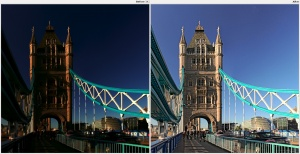
\includegraphics[width=.75\textwidth]{media/300px-Rt407-ba-tonemapping-hdr-cropped.jpg}
        % \caption{Tonemapping - }
    \end{center}
\end{frame}


\begin{frame}
    \frametitle{Why Parallelize?}
    Tone-mapping is done for images, where there are millions of pixels present.
    This is the perfect opportunity for the GPU Acceleration.
    

\end{frame}

\begin{frame}
    \frametitle{References}
    % use \cite to refer
    \begin{thebibliography}{00}
        \bibitem{compiler-book}{Compiler}
        \bibitem{cit1}{Citation 1}
    \end{thebibliography}    

\end{frame}


\end{document}